\documentclass{article}
% Pacchetti di Codifica e Lingua
\usepackage[utf8]{inputenc}
\usepackage[T1]{fontenc}
\usepackage[italian]{babel}

% Pacchetti Grafici e Diagrammi
\usepackage{graphicx}
\usepackage{tikz}
\usepackage{circuitikz}
\usepackage{tikz-3dplot}
\usetikzlibrary{angles,quotes,arrows.meta, positioning}
\usepackage{pgfplots}
\pgfplotsset{compat=1.18}

% Pacchetti Matematici
\usepackage{amsmath, amssymb, amsthm}

% Pacchetti per Tabelle e Unità di Misura
\usepackage{geometry}
\usepackage{siunitx}
\usepackage{booktabs}
\usepackage{tabularx}
\usepackage{colortbl}
\usepackage{adjustbox}

% Pacchetti per Layout e Formattazione
\usepackage{fancyhdr}
\usepackage{float}
\usepackage{microtype}

% Altri Pacchetti Utili
\usepackage{mdframed}
\usepackage{animate}
\usepackage{ulem}
\usepackage{eurosym}

% Pacchetto enumitem
\usepackage{enumitem}

% Definizioni dei Colori
\definecolor{lightblue}{HTML}{9cd8fc}
\definecolor{myblue}{HTML}{139FE9}
\definecolor{myblack}{HTML}{303030}
\definecolor{mygray}{HTML}{787878}
\definecolor{mywhite}{HTML}{c7c7c7}

%\pagecolor{myblack}
%\color{mywhite}
% Definizione del comando \norm
\newcommand{\norm}[1]{\left\lVert#1\right\rVert}

%\font\nullfont=cmr10 

% Ambienti Personalizzati
\newmdtheoremenv[
    backgroundcolor=orange!10,
    linecolor=myblue,
    linewidth=0pt,
    leftmargin=0pt,
    rightmargin=0pt,
    innerleftmargin=10pt,
    innerrightmargin=10pt,
    innertopmargin=10pt,
    innerbottommargin=10pt,
    nobreak
]{curiosity}{Curiosità}

\newmdtheoremenv[
    font=\normalfont\small,
    linewidth=0pt,
    innerleftmargin=10pt,
    innerrightmargin=10pt,
]{example}{Esempio}

\newmdtheoremenv[
  backgroundcolor=lightblue,
  linecolor=myblue,
  linewidth=1.5pt,
  innertopmargin=10pt,
  innerbottommargin=10pt,
  innerrightmargin=10pt,
  innerleftmargin=10pt,
  nobreak
]{theorem}{Teorema}

\newmdtheoremenv[
  backgroundcolor=gray!10,
  linewidth=0pt,
  innertopmargin=10pt,
  innerbottommargin=10pt,
  innerrightmargin=10pt,
  innerleftmargin=10pt,
  nobreak
]{definition}{Definizione}

\newmdtheoremenv[
  backgroundcolor=gray!10,
  linecolor=myblue,
  linewidth=1.5pt,
  innertopmargin=10pt,
  innerbottommargin=10pt,
  innerrightmargin=10pt,
  innerleftmargin=10pt,
  nobreak
]{proposition}{Proposizione}

% Configurazioni di fancyhdr
\pagestyle{fancy}
\fancyhf{} % Pulisce tutti i campi
\fancyhead[LO]{\nouppercase{\rightmark}} % Titolo della sezione
\renewcommand{\headrulewidth}{0.5pt}
\renewcommand{\footrulewidth}{0pt}

\geometry{a4paper, left=20mm, right=20mm, top=20mm, bottom=20mm}

% Pacchetto Hyperref (inserito per ultimo)
\usepackage{hyperref}
% Additional Packages
\usepackage{xparse,array}

\begin{document}
\begin{titlepage}
    \centering
    \vspace*{1cm} % Aggiunge spazio verticale
    
\includegraphics[width=0.6\textwidth]{src/logo.png} % Inserisci il percorso corretto al file del logo
    \vspace{1.5cm}
    
    \Huge
    \textbf{Informe de Laboratorio de Electrotécnia}
    
    \vspace{0.5cm}
    \LARGE
    Práctica 1
    
    \vspace{1.5cm}
    
    \textbf{Michele Mazza y Juan Repiso}
    
    \vfill
    
    \Large
    Grado en Ingeniería de Sistemas Industriales\\
    Universidad Alfonso X el Sabio\\
    \today
\end{titlepage}
\section{Introducción}
En el informe de laboratorio dado, describimos la investigación de tres circuitos de corriente continua, que tiene como objetivo el estudio adicional de las leyes básicas de la electricidad y el correcto funcionamiento de un instrumento como un multímetro. Antes de proceder al ensamblaje y construcción de los montajes, tomamos las medidas de tres resistencias variables que íbamos a utilizar en el experimento:
\begin{itemize}
    \item $R_1 = 625\ m \Omega$
    \item $R_2 = 10.9\ \Omega$
    \item $R_3 = 28.1\ \Omega$
\end{itemize}
\section{Medidas de securidad}
Siempre se deben de tener en cuenta cuestiones de seguridad al trabajar con electricidad. Algunos de ellos son:
\begin{itemize}
  \item Cuidado en el uso de cables: Directamente no se debe tocar un cable en su extremo. Sin embargo, en ocasiones en que es necesario, los dedos deben hacerlo a través del dorso de la mano para que se pueda evitar que sea enganchada a una parte viva del circuito.
  \item Estado de los equipos y cables: En este contexto, todos los cables y equipos deben descartarse si no están en perfecto estado. Se debe evitar el uso o incluso la creación de cables que no estén en buenas condiciones o que carezcan de recubrimiento, ya que estas condiciones son posibles causas de provocación de cortocircuito o de arcos eléctricos.
  \item Usos incorrectos del multimetro: Un multimetro es un aparato que puede estar definido como un voltimetro, amperímetro y óhmetro que permite hacer muchas tareas. Con razón, la clave es utilizar siempre el modo correcto y utilizar los terminales de forma adecuada o se puede dañar el equipo o no obtener los datos requeridos.
  \item Verificación: A institutos en practicas, se recomienda que antes de alimentar a cualquier circuito, se invite a una profesora o supervisor para comprobar y autorizar la estructura final de todo el proceso.
\end{itemize}




\section{Descripción de los Montajes}
\subsection{Montaje 1}
\begin{figure}[H]
  \centering
  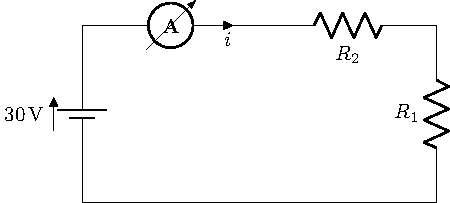
\includegraphics{src/circuit01.pdf}
  \caption{Circuito 1}
  \label{fig:circuit01}
\end{figure}
En el primer circuito, conectamos una fuente de tensión continua de 30 V en serie con un amperímetro (multímetro en modo amperímetro) y las resistencias $R_1$ y $R_2$ en serie.
\subsubsection{Objetivo}
Medir la corriente total que fluye a través del circuito.
\subsubsection{Mediciìon teorica}
La resistencia total del circuito se calcula como la suma de las resistencias $R_1$ y $R_2$:
\begin{equation}
  R_{\text{total}} = R_1 + R_2 = 625\ m \Omega + 10.9\ \Omega = 11.525\ \Omega
\end{equation}
La corriente total del circuito se calcula con la ley de Ohm:
\begin{equation}
  i_{teorica} = \frac{V}{R} = \frac{30\ V}{11.525\ \Omega} \approx 2.604\ A
\end{equation}
\subsubsection{Medición experimental}
Hemos medido a través del amperímetro una $i_{experimental} = 2,56\ A$, que es coherente con el valor teórico considerando posibles errores de medición de los instrumentos.

\subsection{Montaje 2}
\begin{figure}[H]
  \centering
  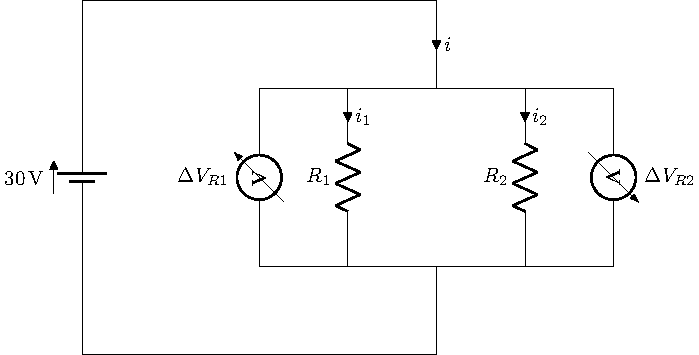
\includegraphics{src/circuit02.pdf}
  \caption{Circuito 2}
  \label{fig:circuit02}
\end{figure}

En el segundo circuito, conectamos el generador de $30\ V$ a dos resistencias, $R_1$ y $R_2$, dispuestas en paralelo. A los extremos de cada resistencia, conectamos un voltímetro para medir la diferencia de potencial.

\subsubsection{Objetivo}
Verificar que la caida de tensión en cada resistencia es igual a la tensión de la fuente.

\subsubsection{Medición teórica}
En un circuito en paralelo, la tensión a través de cada resistencia es igual a la tensión de la fuente:
\begin{equation}
  V_{R1} = V_{R2} = V_{\text{fuente}} = 30\ V
\end{equation}

\subsubsection{Medición experimental}
Hemos medido una diferencia de potencial de $\Delta V_{R1} = 29.77\ V$ y $\Delta V_{R2} = 29.83\ V$, las pequeñas diferencias pueden deberse a caídas de tensión en los cables o a errores instrumentales.

\subsection{Montaje 3}
\begin{figure}[H]
  \centering
  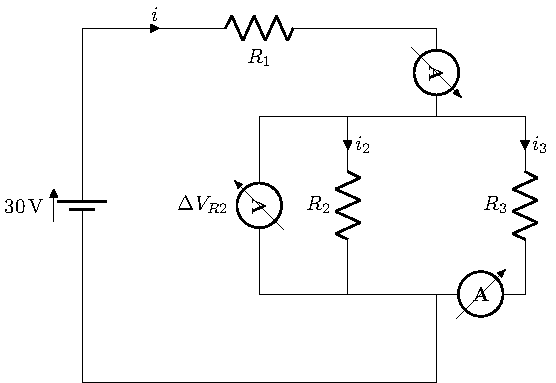
\includegraphics{src/circuit03.pdf}
  \caption{Circuito 3}
  \label{fig:circuit03}
\end{figure}
El tercer circuito consiste en el generador de $30\ V$, un amperímetro en serie y la resistencia $R_1$. Luego, el circuito se divide en dos ramas paralelas: una con la resistencia $R_2$, y otra con la resistencia $R_3$.

\subsubsection{Objetivo}
\begin{itemize}
  \item Medir la corriente total del circuito y las corrientes parciales en cada rama.
  \item Medir la tensión a través de $R_2$.
\end{itemize}

\subsubsection{Medición teórica}
\begin{itemize}
  \item Primero, calculamos la resistencia equivalente de las ramas en paralelo:
\begin{equation}
  \frac{1}{R_{\text{eq}}} = \frac{1}{R_2} + \frac{1}{R_3} 
\end{equation}
\begin{equation}
  R_{\text{eq}} = \frac{R_2 \cdot R_3}{R_2 + R_3} = \frac{10.9\ \Omega \cdot 28.1\ \Omega}{10.9\ \Omega + 28.1\ \Omega} \approx 7.85\ \Omega
\end{equation}
Luego, sumamos $R_{1}$ en serie:
\begin{equation}
  R_{\text{total}} = R_1 + R_{\text{eq}} = 625\ m \Omega + 7.85\ \Omega = 8.475\ \Omega
\end{equation}
La corriente total se calcula con la ley de Ohm:
\begin{equation}
  i_{teorica} = \frac{V}{R} = \frac{30\ V}{8.475\ \Omega} \approx 3.54\ A
\end{equation}
La corriente en la rama con $R_3$ se calcula con un divisor de corriente:
\begin{equation}
  i_{3} = i_{\text{total}} \cdot \frac{R_{2}}{R_2 + R_{3}} = 3.54\ A \cdot \frac{10.9\ \Omega}{10.9\ \Omega + 28.1\ \Omega} \approx 989.38\ mA
\end{equation}
La corriente en la rama con $R_2$ se obtiene por diferencia:
\begin{equation}
  i_{2} = i_{\text{total}} - i_{3} = 3.54\ A - 989.38\ mA = 2.55\ A
\end{equation}
\item La tensión a través de $R_2$ se calcula con la ley de Ohm:
\begin{equation}
  \Delta V_{R2} = i_{2} \cdot R_2 = 2.55\ A \cdot 10.9\ \Omega = 27.79\ V
\end{equation}
\end{itemize}

\subsubsection{Medición experimental}
\begin{itemize}
  \item Hemos medido una corriente total de $i_{\text{total}} = 3.35 A$, una corriente en la rama con $R_3$ de $i_{3} = 0.9 A$ por los limites de medida del amperímetro.
  \item Hemos medido una tensión a través de $R_2$ de $\Delta V_{R2} = 26.71 V$, que es coherente con el valor teórico considerando posibles errores de medición de los instrumentos.
\end{itemize}

\end{document}